\documentclass[tikz,border=8pt]{standalone}
\usepackage{amsmath,amssymb}
\usetikzlibrary{arrows.meta,calc,decorations.markings,decorations.pathmorphing,patterns,shapes.geometric,positioning}

\begin{document}
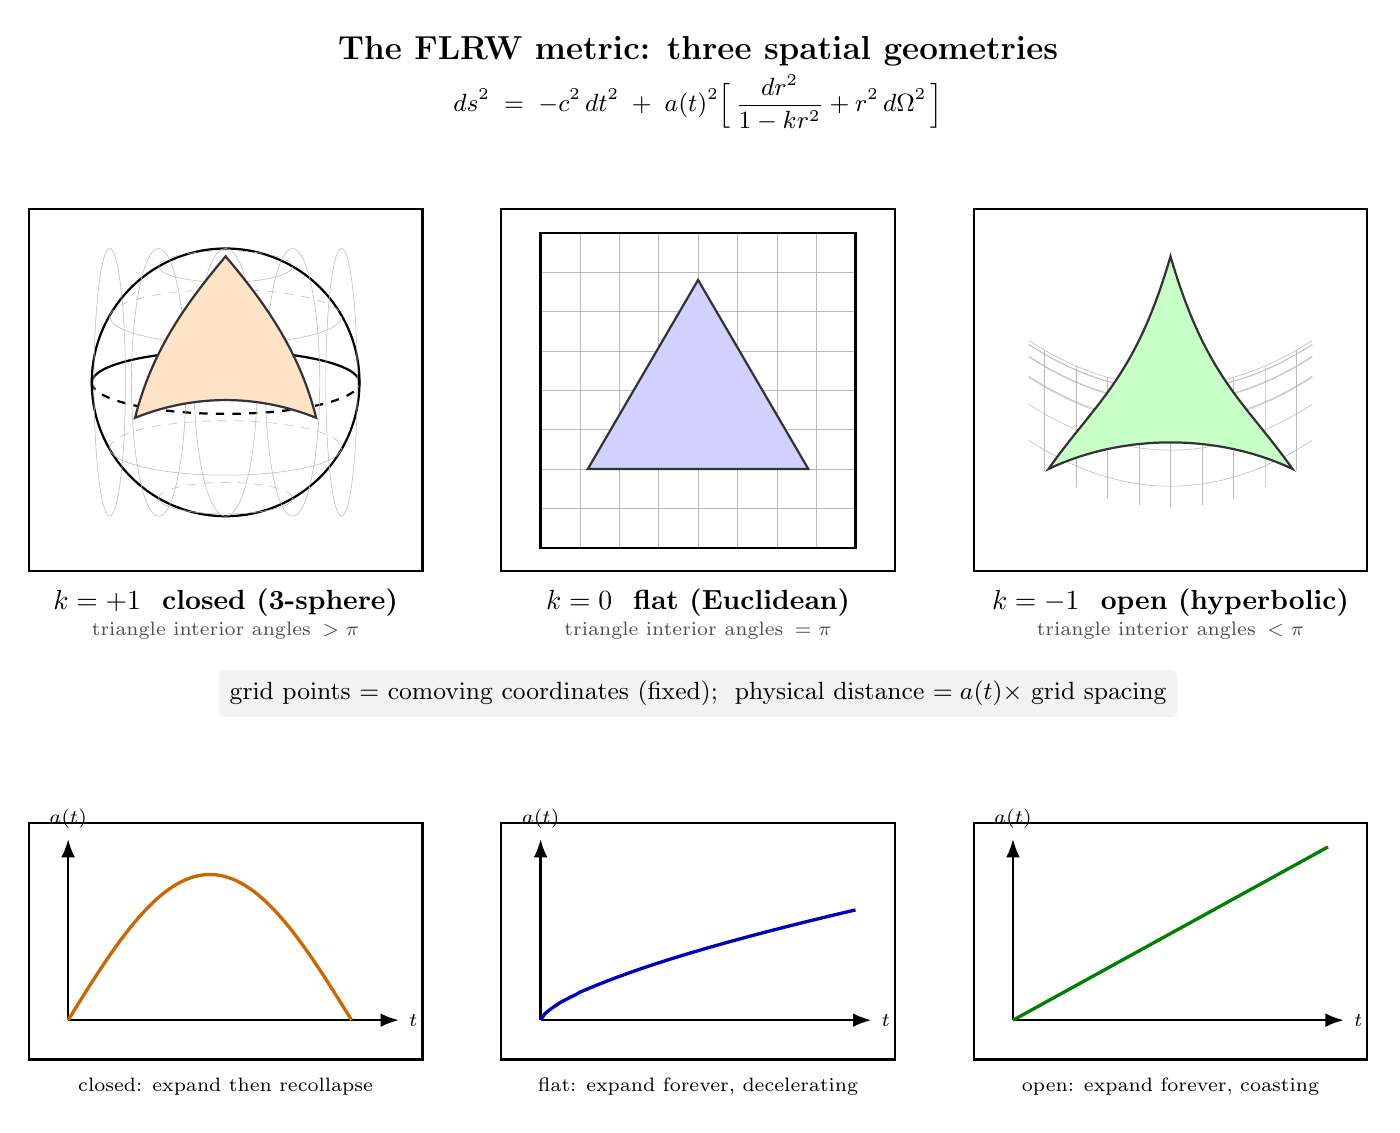
\begin{tikzpicture}[>=Latex,
    panel/.style={rectangle, draw=black, thick, minimum width=5.0cm, minimum height=4.6cm, fill=white},
    smallpanel/.style={rectangle, draw=black, thick, minimum width=5.0cm, minimum height=3.0cm, fill=white},
    triangle3d/.style={fill=orange!22, draw=black!80, thick},
    triangle2d/.style={fill=blue!18, draw=black!80, thick},
    triangleH/.style={fill=green!22, draw=black!80, thick},
    grid3d/.style={draw=gray!55, very thin},
    label/.style={font=\small, align=center}]

  %% =====================================================================
  %% Top header: FLRW metric formula
  %% =====================================================================
  \node[font=\bfseries\large] at (0, 8.7) {The FLRW metric: three spatial geometries};
  \node[font=\small] at (0, 8.05) {%
    $\displaystyle ds^{2} \;=\; -c^{2}\,dt^{2} \;+\; a(t)^{2}\Big[\,\frac{dr^{2}}{1-k r^{2}}+r^{2}\,d\Omega^{2}\,\Big]$%
  };

  %% =====================================================================
  %% Top row: three spatial geometries
  %% =====================================================================

  %% --- Left panel: k = +1 (sphere, closed) -----------------------------
  \begin{scope}[shift={(-6.0, 4.4)}]
    \draw[panel] (-2.5, -2.3) rectangle (2.5, 2.3);

    %% Sphere outline
    \draw[thick, black] (0, 0.1) circle (1.7cm);
    %% Equator (back dashed + front solid)
    \draw[thick, black, dashed] (-1.7, 0.1) arc [start angle=180, end angle=360, x radius=1.7, y radius=0.4];
    \draw[thick, black] (-1.7, 0.1) arc [start angle=180, end angle=0, x radius=1.7, y radius=0.4];

    %% Comoving grid: latitude lines (small/large radius pre-computed)
    %% lat = -60
    \draw[grid3d] (-0.85, -1.371) arc [start angle=180, end angle=360, x radius=0.85, y radius=0.20];
    \draw[grid3d, dashed] (-0.85, -1.371) arc [start angle=180, end angle=0, x radius=0.85, y radius=0.20];
    %% lat = -30
    \draw[grid3d] (-1.472, -0.733) arc [start angle=180, end angle=360, x radius=1.472, y radius=0.346];
    \draw[grid3d, dashed] (-1.472, -0.733) arc [start angle=180, end angle=0, x radius=1.472, y radius=0.346];
    %% lat = 0 (equator already drawn above)
    %% lat = +30
    \draw[grid3d] (-1.472, 0.933) arc [start angle=180, end angle=360, x radius=1.472, y radius=0.346];
    \draw[grid3d, dashed] (-1.472, 0.933) arc [start angle=180, end angle=0, x radius=1.472, y radius=0.346];
    %% lat = +60
    \draw[grid3d] (-0.85, 1.571) arc [start angle=180, end angle=360, x radius=0.85, y radius=0.20];
    \draw[grid3d, dashed] (-0.85, 1.571) arc [start angle=180, end angle=0, x radius=0.85, y radius=0.20];

    %% Longitude lines
    \draw[grid3d] (-1.472, 0.1) ellipse [x radius=0.20, y radius=1.7];
    \draw[grid3d] (-0.85, 0.1) ellipse [x radius=0.346, y radius=1.7];
    \draw[grid3d] (0, 0.1) ellipse [x radius=0.4, y radius=1.7];
    \draw[grid3d] (0.85, 0.1) ellipse [x radius=0.346, y radius=1.7];
    \draw[grid3d] (1.472, 0.1) ellipse [x radius=0.20, y radius=1.7];

    %% Geodesic triangle (spherical: bulging arcs)
    \draw[triangle3d] (0, 1.7) .. controls (-0.55, 1.05) and (-0.95, 0.45) .. (-1.15, -0.35)
      .. controls (-0.4, -0.05) and (0.4, -0.05) .. (1.15, -0.35)
      .. controls (0.95, 0.45) and (0.55, 1.05) .. (0, 1.7) -- cycle;

    %% Title
    \node[label, font=\bfseries] at (0, -2.7) {$k=+1$ \ closed (3-sphere)};
    \node[label, font=\scriptsize, text=black!70] at (0, -3.05) {triangle interior angles $\,>\pi$};
  \end{scope}

  %% --- Middle panel: k = 0 (Euclidean, flat) ---------------------------
  \begin{scope}[shift={(0, 4.4)}]
    \draw[panel] (-2.5, -2.3) rectangle (2.5, 2.3);

    %% Comoving grid: square mesh
    \foreach \i in {-2, -1.5, ..., 2} {
      \draw[grid3d] (\i, -2) -- (\i, 2);
      \draw[grid3d] (-2, \i) -- (2, \i);
    }
    %% Frame the inner region
    \draw[thick, black] (-2, -2) rectangle (2, 2);

    %% Flat triangle
    \draw[triangle2d] (-1.4, -1.0) -- (1.4, -1.0) -- (0.0, 1.4) -- cycle;

    %% Title
    \node[label, font=\bfseries] at (0, -2.7) {$k=0$ \ flat (Euclidean)};
    \node[label, font=\scriptsize, text=black!70] at (0, -3.05) {triangle interior angles $\,=\pi$};
  \end{scope}

  %% --- Right panel: k = -1 (saddle, open) ------------------------------
  \begin{scope}[shift={(6.0, 4.4)}]
    \draw[panel] (-2.5, -2.3) rectangle (2.5, 2.3);

    %% Saddle: stylized hyperboloid (saddle surface)
    %% Draw as a perspective view of a saddle z = x^2 - y^2
    %% horizontal grid lines (constant y)
    \foreach \yy in {-1.6, -1.2, -0.8, -0.4, 0, 0.4, 0.8, 1.2, 1.6} {
      \draw[grid3d, smooth, samples=30, domain=-1.8:1.8] plot (\x, {0.18*(\x*\x) - 0.32*(\yy*\yy) + 0.25*\yy});
    }
    %% vertical grid lines (constant x)
    \foreach \xx in {-1.6, -1.2, -0.8, -0.4, 0, 0.4, 0.8, 1.2, 1.6} {
      \draw[grid3d, smooth, samples=30, domain=-1.8:1.8] plot ({\xx + 0*\x}, {0.18*(\xx*\xx) - 0.32*(\x*\x) + 0.25*\x});
    }

    %% Hyperbolic triangle: vertices on the saddle surface, edges curve INWARD
    %% (sides of a hyperbolic triangle bow inward, sum of angles < pi)
    \coordinate (HA) at (0, 1.7);
    \coordinate (HB) at (-1.55, -1.0);
    \coordinate (HC) at (1.55, -1.0);
    \draw[triangleH] (HA) .. controls (-0.45, 0.15) and (-0.95, -0.15) .. (HB)
      .. controls (-0.6, -0.55) and (0.6, -0.55) .. (HC)
      .. controls (0.95, -0.15) and (0.45, 0.15) .. (HA) -- cycle;

    %% Title
    \node[label, font=\bfseries] at (0, -2.7) {$k=-1$ \ open (hyperbolic)};
    \node[label, font=\scriptsize, text=black!70] at (0, -3.05) {triangle interior angles $\,<\pi$};
  \end{scope}

  %% =====================================================================
  %% Comoving grid annotation (between top and bottom rows)
  %% =====================================================================
  \node[font=\small, align=center, fill=gray!10, inner sep=4pt, rounded corners=2pt]
    at (0, 0.55) {%
    grid points = comoving coordinates (fixed); \ physical distance $=a(t)\times$ grid spacing%
  };

  %% =====================================================================
  %% Bottom row: a(t) curves for three k values
  %% =====================================================================

  %% --- Bottom-left: closed a(t) ----------------------------------------
  \begin{scope}[shift={(-6.0, -2.6)}]
    \draw[smallpanel] (-2.5, -1.5) rectangle (2.5, 1.5);

    %% Axes
    \draw[->, thick] (-2.0, -1.0) -- (2.2, -1.0) node[right, font=\scriptsize] {$t$};
    \draw[->, thick] (-2.0, -1.0) -- (-2.0, 1.3) node[above, font=\scriptsize] {$a(t)$};

    %% Closed: rises and falls (Big Bang -> Big Crunch)
    \draw[very thick, orange!80!black, smooth, samples=80, domain=0:3.6]
      plot ({-2.0+\x}, {-1.0 + 1.85*sin(50*\x)});

    \node[font=\scriptsize, align=center] at (0, -1.85) {closed: expand then recollapse};
  \end{scope}

  %% --- Bottom-middle: flat a(t) ----------------------------------------
  \begin{scope}[shift={(0, -2.6)}]
    \draw[smallpanel] (-2.5, -1.5) rectangle (2.5, 1.5);

    %% Axes
    \draw[->, thick] (-2.0, -1.0) -- (2.2, -1.0) node[right, font=\scriptsize] {$t$};
    \draw[->, thick] (-2.0, -1.0) -- (-2.0, 1.3) node[above, font=\scriptsize] {$a(t)$};

    %% Flat: a ~ t^{2/3} (matter) decelerating, never recollapse
    \draw[very thick, blue!75!black, smooth, samples=80, domain=0:4.0]
      plot ({-2.0+\x}, {-1.0 + 1.4*pow(\x/4.0, 0.667)});

    \node[font=\scriptsize, align=center] at (0, -1.85) {flat: expand forever, decelerating};
  \end{scope}

  %% --- Bottom-right: open a(t) -----------------------------------------
  \begin{scope}[shift={(6.0, -2.6)}]
    \draw[smallpanel] (-2.5, -1.5) rectangle (2.5, 1.5);

    %% Axes
    \draw[->, thick] (-2.0, -1.0) -- (2.2, -1.0) node[right, font=\scriptsize] {$t$};
    \draw[->, thick] (-2.0, -1.0) -- (-2.0, 1.3) node[above, font=\scriptsize] {$a(t)$};

    %% Open: roughly linear, expanding faster
    \draw[very thick, green!50!black, smooth, samples=80, domain=0:4.0]
      plot ({-2.0+\x}, {-1.0 + 0.55*\x});

    \node[font=\scriptsize, align=center] at (0, -1.85) {open: expand forever, coasting};
  \end{scope}

\end{tikzpicture}
\end{document}
